% Options for packages loaded elsewhere
\PassOptionsToPackage{unicode}{hyperref}
\PassOptionsToPackage{hyphens}{url}
\PassOptionsToPackage{dvipsnames,svgnames,x11names}{xcolor}
%
\documentclass[
  letterpaper,
  authoryear]{elsarticle}

\usepackage{amsmath,amssymb}
\usepackage{iftex}
\ifPDFTeX
  \usepackage[T1]{fontenc}
  \usepackage[utf8]{inputenc}
  \usepackage{textcomp} % provide euro and other symbols
\else % if luatex or xetex
  \usepackage{unicode-math}
  \defaultfontfeatures{Scale=MatchLowercase}
  \defaultfontfeatures[\rmfamily]{Ligatures=TeX,Scale=1}
\fi
\usepackage{lmodern}
\ifPDFTeX\else  
    % xetex/luatex font selection
\fi
% Use upquote if available, for straight quotes in verbatim environments
\IfFileExists{upquote.sty}{\usepackage{upquote}}{}
\IfFileExists{microtype.sty}{% use microtype if available
  \usepackage[]{microtype}
  \UseMicrotypeSet[protrusion]{basicmath} % disable protrusion for tt fonts
}{}
\makeatletter
\@ifundefined{KOMAClassName}{% if non-KOMA class
  \IfFileExists{parskip.sty}{%
    \usepackage{parskip}
  }{% else
    \setlength{\parindent}{0pt}
    \setlength{\parskip}{6pt plus 2pt minus 1pt}}
}{% if KOMA class
  \KOMAoptions{parskip=half}}
\makeatother
\usepackage{xcolor}
\setlength{\emergencystretch}{3em} % prevent overfull lines
\setcounter{secnumdepth}{5}
% Make \paragraph and \subparagraph free-standing
\ifx\paragraph\undefined\else
  \let\oldparagraph\paragraph
  \renewcommand{\paragraph}[1]{\oldparagraph{#1}\mbox{}}
\fi
\ifx\subparagraph\undefined\else
  \let\oldsubparagraph\subparagraph
  \renewcommand{\subparagraph}[1]{\oldsubparagraph{#1}\mbox{}}
\fi


\providecommand{\tightlist}{%
  \setlength{\itemsep}{0pt}\setlength{\parskip}{0pt}}\usepackage{longtable,booktabs,array}
\usepackage{calc} % for calculating minipage widths
% Correct order of tables after \paragraph or \subparagraph
\usepackage{etoolbox}
\makeatletter
\patchcmd\longtable{\par}{\if@noskipsec\mbox{}\fi\par}{}{}
\makeatother
% Allow footnotes in longtable head/foot
\IfFileExists{footnotehyper.sty}{\usepackage{footnotehyper}}{\usepackage{footnote}}
\makesavenoteenv{longtable}
\usepackage{graphicx}
\makeatletter
\def\maxwidth{\ifdim\Gin@nat@width>\linewidth\linewidth\else\Gin@nat@width\fi}
\def\maxheight{\ifdim\Gin@nat@height>\textheight\textheight\else\Gin@nat@height\fi}
\makeatother
% Scale images if necessary, so that they will not overflow the page
% margins by default, and it is still possible to overwrite the defaults
% using explicit options in \includegraphics[width, height, ...]{}
\setkeys{Gin}{width=\maxwidth,height=\maxheight,keepaspectratio}
% Set default figure placement to htbp
\makeatletter
\def\fps@figure{htbp}
\makeatother

% These are extra latex packages that the document depends on
% 
\usepackage{siunitx}
\usepackage{booktabs}
\usepackage{longtable}
\usepackage{array}
\usepackage{multirow}
\usepackage{wrapfig}
\usepackage{float}
\usepackage{colortbl}
\usepackage{pdflscape}
\usepackage{tabu}
\usepackage{threeparttable}
\usepackage{threeparttablex}
\usepackage[normalem]{ulem}
\usepackage{makecell}
\usepackage{xcolor}
\makeatletter
\@ifpackageloaded{bookmark}{}{\usepackage{bookmark}}
\makeatother
\makeatletter
\@ifpackageloaded{caption}{}{\usepackage{caption}}
\AtBeginDocument{%
\ifdefined\contentsname
  \renewcommand*\contentsname{Table of contents}
\else
  \newcommand\contentsname{Table of contents}
\fi
\ifdefined\listfigurename
  \renewcommand*\listfigurename{List of Figures}
\else
  \newcommand\listfigurename{List of Figures}
\fi
\ifdefined\listtablename
  \renewcommand*\listtablename{List of Tables}
\else
  \newcommand\listtablename{List of Tables}
\fi
\ifdefined\figurename
  \renewcommand*\figurename{Figure}
\else
  \newcommand\figurename{Figure}
\fi
\ifdefined\tablename
  \renewcommand*\tablename{Table}
\else
  \newcommand\tablename{Table}
\fi
}
\@ifpackageloaded{float}{}{\usepackage{float}}
\floatstyle{ruled}
\@ifundefined{c@chapter}{\newfloat{codelisting}{h}{lop}}{\newfloat{codelisting}{h}{lop}[chapter]}
\floatname{codelisting}{Listing}
\newcommand*\listoflistings{\listof{codelisting}{List of Listings}}
\makeatother
\makeatletter
\makeatother
\makeatletter
\@ifpackageloaded{caption}{}{\usepackage{caption}}
\@ifpackageloaded{subcaption}{}{\usepackage{subcaption}}
\makeatother
\journal{Transportation Research Part A}
\ifLuaTeX
  \usepackage{selnolig}  % disable illegal ligatures
\fi
\usepackage[]{natbib}
\bibliographystyle{elsarticle-harv}
\usepackage{bookmark}

\IfFileExists{xurl.sty}{\usepackage{xurl}}{} % add URL line breaks if available
\urlstyle{same} % disable monospaced font for URLs
\hypersetup{
  pdftitle={Evaluating the effectiveness of an Incident Management Team expansion in Utah},
  pdfauthor={Joel Hyer; Grant Schultz; Gregory S. Macfarlane; Dennis Eggett},
  colorlinks=true,
  linkcolor={blue},
  filecolor={Maroon},
  citecolor={Blue},
  urlcolor={Blue},
  pdfcreator={LaTeX via pandoc}}

\setlength{\parindent}{6pt}
\begin{document}

\begin{frontmatter}
\title{Evaluating the effectiveness of an Incident Management Team
expansion in Utah}
\author[1]{Joel Hyer%
%
}

\author[1]{Grant Schultz%
%
}

\author[1]{Gregory S. Macfarlane%
%
}
 \ead{gregmacfarlane@gmail.com} 
\author[2]{Dennis Eggett%
%
}


\affiliation[1]{organization={Civil and Construction Engineering
Department, Brigham Young University},addressline={430
EB},city={Provo},postcode={84602},postcodesep={}}
\affiliation[2]{organization={Statistics Department, Brigham Young
University},city={Provo},postcode={84602},postcodesep={}}

\cortext[cor1]{Corresponding author}




        
\begin{abstract}
The abstract is a crucial component of any scientific paper, as it
provides a summary of the research and its main findings. This paper
provides guidelines for writing an effective scientific abstract. The
first step is to identify the key elements of the research, such as the
research question, methods, results, and conclusions. Next, the abstract
should be written in a clear and concise manner, using simple language
and avoiding technical jargon. The abstract should also be structured,
with a clear introduction, methods section, results section, and
conclusion. Additionally, the abstract should accurately and succinctly
convey the main findings of the research, highlighting the significance
and implications of the work. By following these guidelines, researchers
can ensure that their abstract effectively communicates the key aspects
of their research and attracts the attention of potential readers. -
Written by ChatGPT
\end{abstract}





\end{frontmatter}
    
\bookmarksetup{startatroot}

\section*{Preface}\label{preface}
\addcontentsline{toc}{section}{Preface}

\markboth{Preface}{Preface}

This is a template repository that I and my students can use to start
projects that will implement the workflow presented in my
\href{https://gregmacfarlane.github.io/lab/workflow.html}{lab
documentation}. It also serves as an instruction manual in this
workflow, a template article, and a sandbox for me to practice and
learn. I encourage students to use the
\href{https://quarto.org/docs/guide/}{Quarto Guide} as their primary
reference.

The document in this template renders to two\footnote{I hope to make it
  possible to render the article to a BYU Engineering thesis as well.
  Give me a bit of time.} outputs:

\begin{itemize}
\item
  A website
\item
  An Elsevier journal article
\end{itemize}

To render this document, use the command \texttt{quarto\ render} in your
terminal pointed at the working directory. This will create a website
available locally in a \texttt{\_book} folder and a PDF of the article
stored in that folder.

To render your website \emph{and} push its content to a live website,
use the command \texttt{quarto\ publish\ gh-pages}. Details of this
process are available on the
\href{https://quarto.org/docs/publishing/github-pages.html\#publish-command}{Quarto
guide}.

You can change the article to a different publisher by following the
directions at the \href{https://github.com/quarto-journals}{Quarto
Journal Templates GitHub} repository.

\bookmarksetup{startatroot}

\section{Introduction}\label{introduction}

The purpose of this report is to present the findings of the regression
analysis for the expansion of the Utah Department of Transportation
(UDOT) Incident Management Team (IMT) program and to determine the
effect of pertinent variables of crash data on IMT performance and user
impacts. In 2019, the Utah Department of Transportation (UDOT) funded a
research study to evaluate the effectiveness of an expanded Incident
Management Team (IMT) program. The number of IMTs patrolling Utah
roadways increased from 13 to 25 between 2018 and 2020. Crash data were
collected from the Utah Highway Patrol's (UHP) Computer-Aided Dispatch
(CAD) database and from the UDOT TransSuite database for 2018 and 2020.
Data were collected to compare IMT performance measures and the user
impacts of crashes responded to by IMTs for both years to evaluate the
benefits of the expanded IMT program. However, these data were
compromised due to the effects of the COVID-19 pandemic.

Because of the unusually low traffic volumes experienced during the
COVID-19 pandemic, one of the recommendations from the research was to
collect data in a future year without the impacts of COVID-19. The
research presented in this report collected data for 2022 using the same
methodology as the previous research to compare IMT performance measures
and user impacts of crashes in 2022 with those of 2018 after traffic
volumes had returned to a similar level as those of pre-pandemic levels.
The performance measures collected include IMT Response Time (RT),
Roadway Clearance Time (RCT), and IMT Incident Clearance Time (ICT). The
study also included the performance measures of UHP RT and UHP ICT but
focused primarily on IMT performance measures rather than those of UHP
units. The user impacts quantified include the affected volume (AV) of
vehicles, excess travel time (ETT) -- or the total delay experienced by
all roadway users in a crash, and excess user cost (EUC) -- or the time
cost of the delay experienced by all roadway users.

There have been many studies conducted on the benefits of incident
management, the potential of large crash data sets to improve ITS
capabilities, using machine learning as well as advanced statistical
methods to predict incident duration, and estimate generally the reduced
delay for incidents which IMTs responded to. However, few studies have
been conducted to quantify the user impacts of incidents responded to by
IMTs using detailed crash and lane closure data to understand the
correlations between specific user impacts and IMT performance measures
as well as other crash variables. Relating these variables using
detailed incident data allows the benefits of IMTs to be more fully
understood as well as guide the allocation of resources to allow highway
agencies to decrease the delay and improve the safety experienced by
roadway users. The effect of IMT program size is also a variable which
has not been specifically addressed.

This manuscript presents a comparison of IMT performance measures and
the user impacts of crashes responded to by IMTs for before the program
expansion (2018) and after the program expansion (2022). The sections
included are a literature review of previous studies, the methods used
to obtain and clean crash data for regression analysis, the results of
the regression analysis, and the conclusions of the results.

\bookmarksetup{startatroot}

\section{Literature Review}\label{literature-review}

Previous studies on traffic incident management have explored the
effectiveness of the positive effect of IMT program policies on traffic
operations and user safety, identifying available data sources used to
obtain and quantify IMT performance measures, compiling large data sets
for use in ITS to improve crash response, using machine learning and
statistical models to predict incident duration occurrence, the
development of traffic simulation models based on incident probability
to optimize the location of IMTs and quantify delay, and estimate the
reduction in delay generally when IMTs respond to a crash.

One study created an open-source platform called DataFITS to collect and
fuse traffic-related data (such as volumes, speeds, weather, etc.) from
different sources to enhance the coverage and quality of data available
to agencies in order to increase the quantity, reliability, and possible
applications of ITS \citep{zisner_datafits_2023}. One application for
which the heterogeneous data fusion was used for was predicting the
speed and volume of traffic in two cities in Germany based on historical
data for multiple types of roadways and under different conditions using
a polynomial regression model, which yielded models with R-squared
values of up to 0.91 for predicting traffic speed and 0.81 for traffic
volume. The other application was an incident classification model that
would first evaluate traffic data using an algorithm to classify the
binary condition of incident or non-incident based on historical data,
which had an accuracy of approximately 90 percent, and then to classify
the traffic condition as being an incident, congestion, or non-incident,
which had an accuracy of approximately 80 percent. This application is
an example of the power of having large data sets available to agencies
to improve incident response and expand the possibilities of ITS
applications.

A study conducted by researchers at Iowa State University ranked
agencies within the state of Iowa based on the effectiveness of the
agency's response to incidents based on RCT
\citep{mumtarin_traffic_2023}. A robust Tobit regression model was
created for RCT and normalized by controlling for variables that were
conditions outside of the agencies' control including crash severity,
roadway type, weather conditions, lighting conditions, whether the crash
was intersection or interchange related, the kind of intersection or
interchange based on available data, the general cause of the crash, and
whether it occurred in an urban or rural context. The model indicated
that crashes in urban areas were cleared 7.4 minutes faster than those
in rural areas. Most adverse weather conditions such as rain, sleet,
hail, ice, and light snow had no statistically significant relationship
with RCT except for blowing snow and fog/smoke, which increased RCT by
3.3 and 5.2 minutes, respectively. Minor PI crashes, major PI crashes,
and FII crashes were shown to have a greater RCT than PDO crashes by
8.7, 28.5, and 108.8 minutes, respectively.

One study analyzed incident duration through three statistical methods
including fixed-parameter ordinary least squares (OLS) regression,
random effects OLS regression, and quantile regression
\citep{wali_heterogeneity_2022}. The goal of using these statistical
methods was to capture and control for the unobserved heterogeneity of
factors that influence incident duration. This is a very logical
approach due to the inherently random nature of traffic crash incidents
and traffic performance in incident conditions. The purpose of including
the quantile regression method was to subset and analyze the data in
specific ranges including the 25th, 50th, 75th, and 95th percentiles due
to the wide range of incident durations that may be experienced; these
results also are useful for developing different incident response
strategies for large incidents as opposed to medium and small incidents.
Overall, the random effects OLS regression model was selected as the
best model for predicting incident duration, which might be compared
with the results presented in this study as RCT, with an R-squared value
of 0.23. Note that all variables in this study were categorical
variables.

While many of the studies on incident duration did not specify how it
was determined other than through agency-provided data, some studies
defined it as ICT while others integrated the speed of traffic into the
platform to determine when an incident occurred. The variables of RCT,
ICT, and T\textsubscript{7}-T\textsubscript{0} discussed and analyzed
later in this report would be comparable to incident duration. While
this study also seeks to model IMT performance measures, there has been
little work done to model or predict the user impacts of crashes, which
are largely dependent on IMT performance measures as well as other
pertinent crash variables.

The National Cooperative Highway Research Program (NCHRP) released
guidelines on quantifying the benefits of TIM strategies by
\citet{shah_development_2022} which state that the reduction of delay
(synonymous with ETT) of roadway users is one of the principle metrics
used to quantify the effectiveness of an IMT program. Studies therein
used traffic models with assumed incident duration times and IMT RT as
well as the ratio of lanes closed to the total number of lanes to
estimate ETT. Different models found that non-TIM delay is between 1.25
and 2.26 times greater than TIM delay, or the delay when IMTs respond to
a crash as opposed to other agencies. However, the limitations of these
models are that they rely on simulation data and assumed values of IMT
performance measures. Simulations are not able to account for the
inherently random, heterogeneous conditions mentioned by
\citet{wali_heterogeneity_2022} that occur in crash data because
simulations visualize the effects of individual incidents assuming that
traffic flows according to rigid assumptions that will not consistently
match field conditions.

Other studies previously referenced also show that IMT performance
measures vary significantly based on field conditions, for which
in-field data sets should be used to verify varying conditions. While
the studies referenced in \citet{shah_development_2022} explored the
effects of when IMTs were present as opposed to when they were not
present, there have been few studies that have addressed the effect of
an expanded IMT program, which findings could significantly benefit
transportation agencies with an existing IMT program by providing
reference for the benefits of an expansion.

This regression analysis is conducted using detailed, in-field incident
data to model the user impacts of crashes responded to by IMTs in
addition to IMT performance measures for both 2018 and 2022 to better
understand how individual crash variables are correlated with user
impacts in addition to performance measures as well as the effect of an
expanded IMT program.

\bookmarksetup{startatroot}

\section{Methodology}\label{methodology}

To estimate the impact of Utah's IMT program expansion through
regression analysis, UHP CAD crash data and UDOT TransSuite lane
closures data were integrated, IMT performance measures were calculated
for each incident after obtaining all required time stamps, and user
impacts were quantified for each incident with qualifying
characteristics.

\subsection{Crash Dataset Integration}\label{crash-dataset-integration}

The primary crash data source for this analysis was the UHP CAD
database, which includes the timestamps of IMTs and UHPs for each
incident response. UHP provided the research team with a version of the
data with confidential information redacted. The crash types included in
the CAD data are Property Damage Only (PDO), Personal Injury (PI), and
Fatal and Incapacitating Injury (FII). Figure~\ref{fig-TIM_Timeline}
shows the timestamps required to calculate RT, RCT, and ICT. The time
stamps needed for calculating performance measures are
T\textsubscript{1}, T\textsubscript{4}, T\textsubscript{5}, and
T\textsubscript{6}. T\textsubscript{1} corresponds with the time when
the incident was reported. T\textsubscript{2} was assumed to be equal to
T\textsubscript{1} due to most incidents being reported by UHP officers
who patrol for crashes that are then verified by TOC personnel.
T\textsubscript{4} is the time at which responders arrived at the
incident location. T\textsubscript{5} corresponds with the time when all
lanes of traffic were cleared, and T\textsubscript{6} corresponds with
the time when first responders left the site. RT, RCT, and ICT are
calculated by taking the difference of T\textsubscript{4},
T\textsubscript{5}, and T\textsubscript{6} with T\textsubscript{1},
respectively. T\textsubscript{7} is the time at which the flow of
traffic returns approximately to normal flow conditions.

\begin{figure}

\centering{

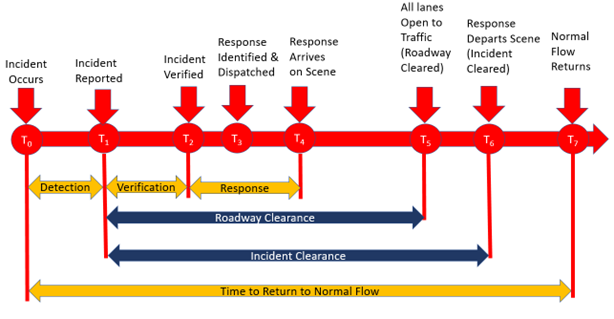
\includegraphics{images/TIM timeline.png}

}

\caption{\label{fig-TIM_Timeline}TIM timeline (adapted from Conklin et
al.~2013).}

\end{figure}%

The CAD data were adequate to determine the performance measures of RT
and ICT for most incidents but not for RCT, which was obtained from the
UDOT TransSuite database which included the time stamps of lane
closures, which were used for the T\textsubscript{5} time stamp for each
incident which TransSuite had the data available. An Excel Visual Basic
for Applications (VBA) script was used to pair incidents from the CAD
data set and TransSuite data set within a similar time frame as
potential matches for the same incident, and potential matches were
evaluated and verified by the research team based on the locations and
details included in both databases for the given incident. The lane
closure data for confirmed matches were then integrated into the CAD
data through a following VBA script.

The total number of incidents contained in the 2018 and 2022 data sets
were 1,097 and 1,526, respectively, which were both taken for the months
of March through August. Of these total incidents, approximately 74 and
66 percent of incidents were PDO crashes for 2018 and 2022,
respectively. PI crashes made up 26 and 34 percent of the total number
of crashes, for 2018 and 2022, respectively, and FII crashes made up
less than 1 percent for both years, as shown in
Table~\ref{tbl-crashdistribution} . This shows a similar crash
distribution between 2018 and 2022 but with a shift to a higher
frequency of PI crashes in 2022 than in 2018.

\begin{longtable}[]{@{}
  >{\centering\arraybackslash}p{(\columnwidth - 8\tabcolsep) * \real{0.2414}}
  >{\centering\arraybackslash}p{(\columnwidth - 8\tabcolsep) * \real{0.1609}}
  >{\centering\arraybackslash}p{(\columnwidth - 8\tabcolsep) * \real{0.2184}}
  >{\centering\arraybackslash}p{(\columnwidth - 8\tabcolsep) * \real{0.1609}}
  >{\centering\arraybackslash}p{(\columnwidth - 8\tabcolsep) * \real{0.2184}}@{}}
\caption{Crash Distribution}\label{tbl-crashdistribution}\tabularnewline
\toprule\noalign{}
\begin{minipage}[b]{\linewidth}\centering
Crash Severity Type
\end{minipage} & \begin{minipage}[b]{\linewidth}\centering
2018 Crashes
\end{minipage} & \begin{minipage}[b]{\linewidth}\centering
2018 Distribution
\end{minipage} & \begin{minipage}[b]{\linewidth}\centering
2022 Crashes
\end{minipage} & \begin{minipage}[b]{\linewidth}\centering
2022 Distribution
\end{minipage} \\
\midrule\noalign{}
\endfirsthead
\toprule\noalign{}
\begin{minipage}[b]{\linewidth}\centering
Crash Severity Type
\end{minipage} & \begin{minipage}[b]{\linewidth}\centering
2018 Crashes
\end{minipage} & \begin{minipage}[b]{\linewidth}\centering
2018 Distribution
\end{minipage} & \begin{minipage}[b]{\linewidth}\centering
2022 Crashes
\end{minipage} & \begin{minipage}[b]{\linewidth}\centering
2022 Distribution
\end{minipage} \\
\midrule\noalign{}
\endhead
\bottomrule\noalign{}
\endlastfoot
FII & 10 & \textless1\% & 9 & \textless1\% \\
PI & 280 & 26\% & 512 & 34\% \\
PDO & 807 & 74\% & 1,005 & 66\% \\
Total & 1,097 & 100\% & 1,526 & 100\% \\
\end{longtable}

\subsection{IMT Performance Measures}\label{imt-performance-measures}

Nearly all incidents had an ICT value and the majority had an RT value,
as shown in Table~\ref{tbl-datatype}. However, only 28 percent of
incidents in 2018 and 21 percent of incidents in 2022 had an available
RCT value. This reduced the total number of incidents with all necessary
time stamps and performance measures (RT, RCT, and ICT) to 283 and 307
incidents for 2018 and 2022, respectively, leaving only 26 percent and
20 percent of the original number of incidents, respectively.

\begin{longtable}[]{@{}
  >{\centering\arraybackslash}p{(\columnwidth - 8\tabcolsep) * \real{0.3737}}
  >{\centering\arraybackslash}p{(\columnwidth - 8\tabcolsep) * \real{0.1414}}
  >{\centering\arraybackslash}p{(\columnwidth - 8\tabcolsep) * \real{0.1717}}
  >{\centering\arraybackslash}p{(\columnwidth - 8\tabcolsep) * \real{0.1414}}
  >{\centering\arraybackslash}p{(\columnwidth - 8\tabcolsep) * \real{0.1717}}@{}}
\caption{Data Type}\label{tbl-datatype}\tabularnewline
\toprule\noalign{}
\begin{minipage}[b]{\linewidth}\centering
Data Type
\end{minipage} & \begin{minipage}[b]{\linewidth}\centering
2018 Crashes
\end{minipage} & \begin{minipage}[b]{\linewidth}\centering
2018 Percentage
\end{minipage} & \begin{minipage}[b]{\linewidth}\centering
2022 Crashes
\end{minipage} & \begin{minipage}[b]{\linewidth}\centering
2022 Percentage
\end{minipage} \\
\midrule\noalign{}
\endfirsthead
\toprule\noalign{}
\begin{minipage}[b]{\linewidth}\centering
Data Type
\end{minipage} & \begin{minipage}[b]{\linewidth}\centering
2018 Crashes
\end{minipage} & \begin{minipage}[b]{\linewidth}\centering
2018 Percentage
\end{minipage} & \begin{minipage}[b]{\linewidth}\centering
2022 Crashes
\end{minipage} & \begin{minipage}[b]{\linewidth}\centering
2022 Percentage
\end{minipage} \\
\midrule\noalign{}
\endhead
\bottomrule\noalign{}
\endlastfoot
Incidents & 1,097 & 100\% & 1,526 & 100\% \\
ICT & 1,089 & 99\% & 1,520 & \textgreater99\% \\
RT & 944 & 86\% & 1,272 & 83\% \\
RCT & 305 & 28\% & 319 & 21\% \\
ICT, RT, and RCT & 283 & 26\% & 307 & 20\% \\
Incidents Analyzed for User Impacts & 172 & 16\% & 236 & 15\% \\
\end{longtable}

The distribution of IMT RT for the years of 2018 and 2022 is shown in
Figure~\ref{fig-RT2018} and Figure~\ref{fig-RT2022}, respectively. The
distribution shifted from 58 percent of incidents responded to within
the first 15 minutes of a crash in 2018 to 62 percent in 2022, yielding
a percent difference of approximately 7 percent between the two years.
This shows that IMTs responded slightly faster to incidents in 2022
after the program expansion, likely due to having more teams to respond
to more crashes more quickly.

\begin{figure}

\centering{

\captionsetup{labelsep=none}\includegraphics{03_methods_files/figure-pdf/fig-RT2018-1.pdf}

}

\caption{\label{fig-RT2018}}

\end{figure}%

\begin{figure}

\centering{

\captionsetup{labelsep=none}\includegraphics{03_methods_files/figure-pdf/fig-RT2022-1.pdf}

}

\caption{\label{fig-RT2022}}

\end{figure}%

The distribution of IMT RCT for the years of 2018 and 2022 is shown in
Figure~\ref{fig-RCT2018} and Figure~\ref{fig-RCT2022}, respectively. The
distribution shifted from 19 percent of incidents for which IMTs cleared
all lanes of traffic within the first 45 minutes in 2018 to 13 percent
of incidents in 2022, showing a percent decrease of approximately 32
percent between the two years, and that IMTs took longer to clear all
lanes in 2022 than in 2018. While the reason for this is indefinite, the
greater percentage of PI crashes in 2022 (34 percent) than in 2018 (26
percent) is a likely cause for longer RCTs in 2022 than in 2018. It was
also observed for a previous UDOT study collecting 2020 crash data using
the same methodology that IMT RCT was also longer in 2020 than in 2018
as noted in \citet{schultz_analysis_2023}. It was hypothesized that IMTs
placed a higher priority on safety while aiding crash victims during the
COVID-19 pandemic in 2020.

\begin{figure}

\centering{

\captionsetup{labelsep=none}\includegraphics{03_methods_files/figure-pdf/fig-RCT2018-1.pdf}

}

\caption{\label{fig-RCT2018}}

\end{figure}%

\begin{figure}

\centering{

\captionsetup{labelsep=none}\includegraphics{03_methods_files/figure-pdf/fig-RCT2022-1.pdf}

}

\caption{\label{fig-RCT2022}}

\end{figure}%

It was found that some RCT values were greater than their respective ICT
values, which conceptually is invalid because IMTs should not have left
the crash site before the roadway was cleared. It was assumed that
because CAD timestamps are reported by UHP teams that are on site during
an incident and the other data points come from the CAD dataset, the CAD
data would be more reliable in this case than TransSuite data. In these
cases, the ICT value of the incident was substituted for the RCT value.
The RCT values that were greater than their respective ICT values were
usually within 10 minutes or less of the ICT value, so the potential
error could have also been due to TOC operators having multiple
incidents to watch and other urgent tasks that could have kept them busy
until they detected that the incident had been cleared from CCTV
footage. It is also possible that IMTs and UHP officers reported leaving
the site sooner than they actually did. This effect of replacing RCTs
with their respective ICT in cases where RCT was greater than ICT only
shifted the distribution of RCT from the unmodified data values by about
1 percent, so the effects of crashes with this discrepancy were
considered to be insignificant.

The distribution of IMT ICT for years 2018 and 2022 is shown in
Figure~\ref{fig-ICT2018} and Figure~\ref{fig-ICT2022}, respectively. The
distribution of IMT ICT shifted from IMTs clearing a given crash and
leaving the site within the first 45 minutes of a given incident for 61
percent of incidents in 2018 to 67 percent of incidents in 2022. This
reflects a percent difference of 10 percent and shows that in spite of
IMTs not necessarily clearing the lanes of the roadway more quickly in
2022 than in 2018 that they still concluded their work at an incident
overall more quickly in 2022 than in 2018, which is likely due to the
increase in IMTs able to aid in crash response.

\begin{figure}

\centering{

\captionsetup{labelsep=none}\includegraphics{03_methods_files/figure-pdf/fig-ICT2018-1.pdf}

}

\caption{\label{fig-ICT2018}}

\end{figure}%

\begin{figure}

\centering{

\captionsetup{labelsep=none}\includegraphics{03_methods_files/figure-pdf/fig-ICT2022-1.pdf}

}

\caption{\label{fig-ICT2022}}

\end{figure}%

\subsection{User Impacts}\label{user-impacts}

As mentioned previously, the user impacts quantified in this study are
AV, ETT, and EUC, and the number of incidents for which user impacts
could be evaluated was 172 and 236 for years 2018 and 2022,
respectively. The criteria that incidents were required to meet in order
to be evaluated for user impacts were as follows:

\begin{enumerate}
\def\labelenumi{\arabic{enumi}.}
\item
  There was a decipherable queue
\item
  There were no secondary incidents whose queue affected that of the
  incident being evaluated
\item
  There were sufficient traffic data to perform the analysis.
\end{enumerate}

The traffic data included as part of the analysis were speed and volumes
taken from the PeMS database and speed and average travel time for
individual routes taken from the Clear Guide (previously iPeMS)
database. The PeMS data are collected through loop detectors and the
Clear Guide data are collected through probe data taken from cell phone
applications and in-vehicle GPS units.

The general process for calculating user impacts of incidents where IMTs
are present requires establishing a baseline of normal traffic
conditions to compare with incident traffic conditions. Therefore, three
days with normal traffic conditions for the same time period and
location as the incident are chosen to compare with incident traffic
conditions. As shown previously in Figure~\ref{fig-TIM_Timeline} ,
T\textsubscript{0} is the time at which an incident occurs and
T\textsubscript{7} is the time at which traffic conditions return to
normal. The difference between T\textsubscript{7} and T\textsubscript{0}
(T\textsubscript{7}-T\textsubscript{0}) represents the amount of time
which the average speed of traffic was significantly below normal and
roadway users experienced significant delays.

The exact time at which an incident occurred was not contained in the
crash data, and the PeMS speed and volume data have a limited
granularity of 5 minutes. Therefore, T\textsubscript{0} was determined
to be the first 5-minute increment for which the average speed of
traffic was reduced significantly below normal, and T\textsubscript{7}
was determined to be the first 5-minute increment for which the average
speed of traffic returned to within the same threshold of normal
traffic. For the purposes of this study, the threshold of normal traffic
conditions was within 20 mph of the average speed of the average of
normal days. In cases where incidents did not have a reduction in speed
of 20 mph or more, a lower difference in the average speed of traffic
was determined by the research team. While this process introduces
subjectivity to the analysis process, the threshold of within 20 mph of
traffic was meant to be a conservative estimate.

The volume of vehicles that diverted to other routes due to congestion
caused by an incident was not quantified as part of the AV of an
incident. To accurately quantify AV with some vehicles diverting and
exiting the roadway during the incident, the section of the roadway that
was affected by the crash was segmented into links (called subroutes)
between ramps. The AV of each subroute was measured as the sum of the
volume of vehicles between T\textsubscript{0} and T\textsubscript{7} for
the incident day, and the AV of the incident was taken to be the maximum
AV of all subroutes affected by the crash. For cases when severe crashes
occurred and traffic was diverted to other routes, the incident was not
quantified. The ETT of an incident was found by calculating the ETT for
each 5-minute increment between T\textsubscript{0} and
T\textsubscript{7} for the incident and average of normal days. The
hours of ETT for each 5-minute increment were found by multiplying the
average travel time of the subroute by the volume of vehicles at that
loop detector. The ETT of an incident was then calculated by taking the
difference between the sum of the ETT for each 5-minute increment
between T\textsubscript{0} and T\textsubscript{7} for the incident and
average of normal days.

The EUC is the sum of the cost of travel time for passenger vehicles and
trucks. Costs due to the ETT of passengers and trucks are the only
factors considered in this analysis, and the costs of excess fuel
burned, property damage of a crash, injuries if sustained during the
crash, and the impacts of motor vehicle emissions on public health are
not included in this study, making EUC values for this study a
conservative estimate. To account for the difference in cost of travel
time for trucks from that of passenger vehicles, the percentage of
trucks in traffic was obtained from PeMS and separate hourly costs were
used for passenger vehicles and trucks. The percentage of trucks in
traffic (Truck\%) for this study was based on the percentage of vehicles
that were 30 ft or longer while those that were less than 30 ft were
passenger vehicles. The percentage of trucks was taken from the same
loop detector as that of the AV of the incident.

The individual hourly cost (IHC) was estimated to be \$17.81 and the
truck hourly cost (THC) was estimated to be \$53.69 based on a study by
the Texas A\&M Transportation Institute \citep{ellis_value_2017} . While
these values are outdated for 2022 user impacts data, the same values
were used as those for 2018 data during Phase I and Phase II to make a
valid comparison without the effects of inflation as a confounding
factor. The EUC formula also includes an average vehicle occupancy (AVO)
factor to account for the time of multiple passengers per vehicle. THC
has an incorporated AVO of 1.14, thus it does not require an external
AVO factor in the EUC formula. IHC is multiplied by an AVO factor
calibrated to the given interstate, direction of travel, and time of day
for which the incident occurred. These AVO values were obtained from
\citet{schultz_ut1503_2015} and, while the values are somewhat outdated
for 2022 data, were used to be consistent with 2018 data values. The
formula for EUC is shown below: \$\$

EUC = ETT \times ((1- \%~Trucks) \times AVO \times IHC + \%~Trucks
\times THC) \$\$

See \citet{schultz_analysis_2023} for a condensed summary of how user
impacts are quantified and evaluated. The median values of each user
impact are shown below. Because the data is heavily right-skewed due to
some outlier incidents with very large user impact values relative to
most that would skew an average, the median is used as the metric for
comparison. The median user impacts are compared between 2018 and 2022
by crash type in \textbf{?@tbl-PDOUserImpacts},
Table~\ref{tbl-PIUserImpacts}, and Table~\ref{tbl-FIIUserImpacts}.

There is a significant percent difference between user impacts in 2018
and 2022. The percent difference the medians of 2018 and 2022 AV values
is approximately 22 percent, and the percent difference for ETT and EUC
is approximately 44 and 41 percent, respectively. Because EUC is
primarily a function of ETT, it is proportional to and highly correlated
with ETT. The percent difference between 2018 and 2022 AV values for PI
crashes was slightly lower than PDO crashes at 20 percent, but the
percent difference between ETT and EUC values was greater than PDO
crashes with values of approximately 51 percent.

\begin{table}
\centering
\begin{tabular}[t]{c|c|c|c}
\hline
Year & AV & ETT & EUC\\
\hline
2018 & 6477.0 & 327.88 & 8115.92\\
\hline
2022 & 5026.5 & 183.77 & 4757.91\\
\hline
\end{tabular}
\end{table}

\begin{table}

\caption{\label{tbl-PIUserImpacts}Median User Impacts of PI Crashes}

\centering{

\centering
\begin{tabular}[t]{c|c|c|c}
\hline
Year & AV & ETT & EUC\\
\hline
2018 & 6883 & 483.09 & 12672.89\\
\hline
2022 & 5518 & 230.75 & 6215.59\\
\hline
\end{tabular}

}

\end{table}%

Because of the very small sample size of FII crashes for both years, it
should be noted that the median user impact values for this crash type
are highly skewed. The percent difference in AV values for 2018 and 2022
crashes was -22 percent, this being the only user impact to experience
an increase in user impacts between 2018 and 2022. However, the percent
difference in ETT and EUC between 2018 and 2022 FII crashes were both
approximately 93 percent. This indicates that while more vehicles were
affected in 2022 during FII crashes that the actual delay experienced by
each vehicle affected was minor.

\begin{table}

\caption{\label{tbl-FIIUserImpacts}Median User Impacts of FII Crashes}

\centering{

\centering
\begin{tabular}[t]{c|c|c|c}
\hline
Year & AV & ETT & EUC\\
\hline
2018 & 6494.5 & 3600.950 & 97899.53\\
\hline
2022 & 7896.5 & 252.705 & 6615.98\\
\hline
\end{tabular}

}

\end{table}%

\subsection{Models}\label{models}

This study hypothesizes that the expanded IMT program decreased user
impacts as well as IMT RT. The dependent variables considered in this
analysis include all user impacts (Ln AV, Ln ETT, and Ln EUC), IMT
performance measures (IMT RT, Ln RCT, Ln IMT ICT), and Ln UHP ICT. Due
to the data distribution for all user impacts and most performance
measures being right-skewed, or skwewed towards large outliers, it was
determined that a natural log (Ln) transformation would be taken to
better fit the data with the exception of IMT RT, for which an Ln
transformation did not help better describe the data for this variable.
Performance measures were also used as independent variables when user
impacts were analyzed as dependent variables in addition to incident
characteristics. The following incident characteristics were considered
in the models for this analysis:

\begin{itemize}
\item
  Year: The years for which crash data were analyzed were 2018
  (reference case) and 2022, explaining the difference in user impacts
  and IMT performance based on IMT program size before and after the
  expansion. This was treated as a categorical variable.
\item
  Crash Type: This includes PDO, PI, and FII crashes where PI was used
  as the reference case.
\item
  Time Range: The 5 time ranges for which crashes were divided into that
  were as follows:

  \begin{itemize}
  \item
    Morning Off Peak: 11:45 PM to 5:30 AM
  \item
    AM Peak: 5:30 AM to 9:00 AM
  \item
    Afternoon Off Peak (Reference case): 9:00 AM to 3:45 PM
  \item
    PM Peak: 3:45 PM to 6:15 PM
  \item
    Night Off Peak: 6:15 PM to 11:45 PM
  \end{itemize}
\item
  Number of IMTs: The number of IMTs that responded to a crash. Note
  that this is a reactionary variable. IMT protocol was to dispatch one
  team for crash response for most incidents or two teams for more
  severe incidents. Additional teams were sent based on crash severity
  and IMT availability.
\item
  Number of UHPs: The number of UHP teams that responded to a crash.
\item
  Number of Lanes Closed: The total number of lanes closed at any point
  during incident response.
\item
  Time Weighted Number of Lanes Closed (TWNLC): The time weighted
  average of the number of lanes closed during incident response. This
  was calculated to more precisely determine the user impacts of a
  crash. This was calculated using the following formula where t\_i is
  the number of minutes that each given lane i was closed (0 minutes for
  lanes that were not closed), N is the number of lanes at the
  bottleneck of the crash, and t\textsuperscript{*} is the total time
  for which any lane of the roadway was closed during an incident.
\end{itemize}

\[ TWNLC = \frac{\sum_{i=1}^{N}t_i}{N \times t^*}
\]

\begin{itemize}
\tightlist
\item
  Capacity ratio of the roadway: The ratio of the time weighted average
  number of lanes open (or 1 minus TWNLC) to the total number of lanes
  (N) at the bottleneck, as shown in the following formula.
\end{itemize}

\[ Capacity = \frac{N-TWNLC}{N}
\]

\begin{itemize}
\item
  Ln T\textsubscript{7}-T\textsubscript{0}: This is the natural log of
  the difference between the time when the average speed of traffic
  during an incident returned to within 20 mph of the average speed at
  normal conditions (T\textsubscript{7}) and the time when the incident
  occurred (T\textsubscript{0}). This is effectively the incident
  duration for which roadway users are impacted. A logarithmic
  transformation was applied due to the right-skew of the data and to
  acheieve best fit in linear regression.
\item
  Ln T\textsubscript{7}-T\textsubscript{5}: This is the difference
  between the time when the average speed of traffic during an incident
  returned to within 20 mph of the average speed at normal conditions
  (T\textsubscript{7}) and the time when all lanes at the bottleneck of
  the incident were cleared (T\textsubscript{5}). This effectively
  represents the time required for traffic to return to normal after all
  lanes being cleared. A logarithmic transformation was also applied to
  this variable due to the right-skew of the data and to achieve best
  fit in linear regression.
\end{itemize}

One limitation to using the natural log transformation for the Ln
T\textsubscript{7}-T\textsubscript{5} parameter is that for incidents
which had a negative T\textsubscript{7}-T\textsubscript{5} value, this
yielded an undefined value. Approximately 18 percent of incidents
analyzed for used impacts had a negative
T\textsubscript{7}-T\textsubscript{5} value, indicating that the speed
of traffic returned to normal before IMTs finished clearing all lanes of
traffic for approximately 18 percent of incidents. Removing the natural
log transformation for this parameter resulted in a poor fit of the
model with user impacts, so the natural log transformation was used
despite its limitation. An inverse Ln
T\textsubscript{5}-T\textsubscript{7} value to the Ln
T\textsubscript{7}-T\textsubscript{5} value was calculated and analyzed
for the 18 percent of incidents for which
T\textsubscript{7}-T\textsubscript{5} was negative. However, this
parameter was not statistically significant when analyzed as an
independent variable with user impacts as dependent variables.

Therefore, models including the Ln T\textsubscript{7}-T\textsubscript{5}
parameter had to be limited to include only the crashes for which
T\textsubscript{7}-T\textsubscript{5} was greater than zero. For this
purpose, all groups of models which include the Ln
T\textsubscript{7}-T\textsubscript{5} parameter will also include models
within the group that do not include Ln
T\textsubscript{7}-T\textsubscript{5} to also describe the minority of
incidents for which the effects of the crash dissipated before IMTs
finished clearing all lanes.

The model groups analyzed to evaluate the UDOT IMT program expansion are
as follows, \[ 
{Performance Measures}_i = {Year}_i + {Crash Type}_i + X_i\beta
\] and \[ 
{User Impacts}_i = {Year}_i + {CrashType}_i + {TimeRange}_i + PerformanceMeasures + Ln T_7 -T_0 +  X_i\beta
\]

where the variable index \(i\) denotes being for a single incident,
\(X\) is a vector of the other incident characteristics variables not
listed above, and \(\beta\) are estimated coefficients.

\bookmarksetup{startatroot}

\section{Results}\label{results}

The purpose of this section is to present the results of the regression
analysis of the UDOT IMT program expansion. The IMT performance measures
of RT, Ln RCT, and Ln ICT are analyzed with incident characteristics as
independent variables to show the impact of the expansion of the IMT
program as well as other variables that best describe each performance
measure. User impacts of Ln AV, Ln ETT, and Ln EUC are then analyzed
with both performance measures and incident characteristics as
independent variables. Overall, user impacts have many more variables
that explain them with significantly better fit than do performance
measures with the prime variable being Ln
T\textsubscript{7}-T\textsubscript{0}, representing the natural log
transformed total time which an incident significantly decreases the
average speed of traffic.

\subsection{Performance Measures}\label{performance-measures}

The IMT performance measures of RT, Ln RCT, and Ln ICT were analyzed in
a regression analysis against several incident characteristics. Overall,
the program expansion results in minor improvements in RT but not for
RCT and ICT. However, the analysis of performance measures provides
models of comparable to fit to those of robust previous studies such as
\citet{mumtarin_traffic_2023} using continuous variables such as the
number of IMTs, UHP teams, lanes Closed, and the TWNLC as well as
capacity ratio variables, which provide a significantly better overall
fit compared to the non-continuous variables of crash type and time
range, as shown in the models of this subsection.

IMT RT is primarily described by the number of IMTs responding to an
incident and the capacity of the roadway based on the number of lanes
closed as represented by the TWNLC and Capacity ratio variables, which
variables are included in the statistical models in
Table~\ref{tbl-rtmodels}. The year 2018 variable indicates that IMTs
took approximately 2.7 minutes longer to respond to crashes in 2018
before the expansion than in 2022 when there were more units. The number
of IMTs variable indicates that IMT RT decreased by approximately 1.5
minutes for each added IMT that responded to an incident, showing that
crashes where more IMTs were required were treated more urgently after
detection than those where fewer IMTs responded. The TWNLC coefficient
of 1.931 minutes indicates that IMTs took almost 2 minutes longer to
respond for each 1.0 incremental increase in the average numer of lanes
closed throughout the crash. This suggests that IMTs could not reach the
crash site as quickly due to congestion when more lanes were closed.

The capacity ratio variable describes the same phenomenon but is
normalized for the total number of lanes at the bottleneck. A 1.0
decrease in the capacity ratio (from 1.0 to 0) represents TWNLC changing
from no lanes being closed to all lanes being closed, which severely
increases IMT RT. For example, a crash where 1 out of 4 lanes were
closed after an incident occured until cleared by IMTs would have a
capacity ratio of 0.75 and the coefficient (representing the change in
IMT RT based on the ratio) would be 0.75 times -9.856 minutes, or 7.392
minutes less than intercept, where the intercept represents the IMT RT
value for the base condition of a capacity ratio of 0. More lanes closed
for part or all of the duration of an incident increases the average
number of lanes closed for the time period before lanes were reopened -
resulting in a higher RT value. The TWNLC RT model has a significantly
lower intercept than in the capacity ratio RT model, which represents a
high RT value for the base condition of a capacity ratio of 0.

The time range variable was only statistically significant for the
Morning Off Peak range; a coefficient of between 39 and 42 shows that
IMTs took significantly longer to respond to crashes in the early
morning than in the afternoon off peak. The lanes closed and crash type
variables were also analyzed but did not help to improve the fit of the
model or help further explain differing values of IMT RT. A year
2018*Number of IMTs interaction term was analyzed for but was also not
statistically significant.

\begin{table}

\caption{\label{tbl-rtmodels}Estimated Models of IMT RT}

\centering{

\centering
\begin{tabular}[t]{lccc}
\toprule
  & Base & w/ TWNLC & w/ Capacity Ratio\\
\midrule
(Intercept) & 15.657*** & 13.716*** & 23.464***\\
 & (1.423) & (1.662) & (2.808)\\
Year 2018 (ref. 2022) & 2.737** & 2.673* & 2.688**\\
 & (1.009) & (1.040) & (1.037)\\
Morning Off Peak (ref. Afternoon Off Peak) & 42.974*** & 39.110*** & 39.812***\\
 & (4.838) & (5.033) & (4.933)\\
AM Peak (ref. Afternoon Off Peak) & -1.454 & -1.645 & -1.783\\
 & (1.299) & (1.336) & (1.332)\\
PM Peak (ref. Afternoon Off Peak) & 0.643 & 0.117 & -0.027\\
 & (1.179) & (1.219) & (1.216)\\
Night Off Peak (ref. Afternoon Off Peak) & 0.362 & -0.468 & -0.523\\
 & (2.071) & (2.206) & (2.198)\\
N. IMTs & -1.476* & -1.978** & -1.942**\\
 & (0.698) & (0.751) & (0.741)\\
Time Weighted Number of Lanes Closed &  & 1.931** & \\
 &  & (0.692) & \\
Capacity Ratio of Roadway &  &  & -9.856**\\
 &  &  & (3.109)\\
\midrule
Num.Obs. & 384 & 362 & 362\\
R2 & 0.201 & 0.220 & 0.225\\
R2 Adj. & 0.188 & 0.205 & 0.210\\
\bottomrule
\multicolumn{4}{l}{\rule{0pt}{1em}+ p $<$ 0.1, * p $<$ 0.05, ** p $<$ 0.01, *** p $<$ 0.001}\\
\multicolumn{4}{l}{\rule{0pt}{1em}Dependent variable: RT}\\
\multicolumn{4}{l}{\rule{0pt}{1em}Standard errors in parentheses}\\
\end{tabular}

}

\end{table}%

Ln RCT models shown in Table~\ref{tbl-rctmodels} includes the variables
that were found to best explain RCT. The year 2018 variable was found to
be moderately statistically significant; its coefficient explains that
IMT RCT had a multiplicative difference of approximately
e\textsuperscript{-0.17}, or 0.84, between 2018 and 2022 crashes,
showing that IMTs responded to crashes approximately 16 percent faster
in 2018. While the reason for this is not fully explained by these
models, it should be noted that the PDO crash type variables is highly
statistically significant and has a multiplicative difference with the
reference case of PI crashes of approximately e\textsuperscript{-0.4},
or 0.67, showing that PI crashes required approximately 33 percent more
time to clear than PDO crashes.

The other incident characteristics included as independent variables
describing RCT are IMT RT, the number of UHP teams, and the number of
IMTs. Each added minute of RT results in an increase of approximately
e\textsuperscript{0.02}, or 2 percent, in RCT, indicating that IMT RT
incurs minor impacts on RCT. The addition of each UHP team and IMT that
respond to each crash is approximately e\textsuperscript{0.11} and
e\textsuperscript{0.19}, or 1.12 and 1.21, times higher RCT values. The
crash type variable was analyzed but was not statistically significant
and was thus not included in the Ln RCT models.

\begin{table}

\caption{\label{tbl-rctmodels}Estimated Models of RCT}

\centering{

\centering
\begin{tabular}[t]{lccc}
\toprule
  & Ln RCT Base & Ln RCT w/UHPs & Ln RCT w/ all teams\\
\midrule
(Intercept) & 7.619*** & 7.185*** & 6.944***\\
 & (0.080) & (0.114) & (0.134)\\
Year 2018 (ref. 2022) & -0.177* & -0.162* & -0.170*\\
 & (0.082) & (0.079) & (0.078)\\
PDO Crash (ref. PDO) & -0.463*** & -0.393*** & -0.389***\\
 & (0.081) & (0.080) & (0.079)\\
FII crash (ref. PI) & 1.172*** & 0.331 & 0.313\\
 & (0.331) & (0.359) & (0.355)\\
IMT RT & 0.018*** & 0.019*** & 0.020***\\
 & (0.004) & (0.004) & (0.004)\\
N. UHP Teams &  & 0.120*** & 0.101***\\
 &  & (0.023) & (0.024)\\
N. IMTs &  &  & 0.187**\\
 &  &  & (0.056)\\
\midrule
Num.Obs. & 384 & 384 & 384\\
R2 & 0.196 & 0.249 & 0.270\\
R2 Adj. & 0.187 & 0.239 & 0.258\\
\bottomrule
\multicolumn{4}{l}{\rule{0pt}{1em}+ p $<$ 0.1, * p $<$ 0.05, ** p $<$ 0.01, *** p $<$ 0.001}\\
\multicolumn{4}{l}{\rule{0pt}{1em}Dependent variable: Ln RCT}\\
\multicolumn{4}{l}{\rule{0pt}{1em}Standard errors in parentheses}\\
\end{tabular}

}

\end{table}%

IMT ICT models are estimated in Table~\ref{tbl-imtictmodels}. The year
2018 variable is not statistically significant in each of the models,
showing that the expansion of the IMT program does not make a
significant difference on IMT ICT. The independent variables that best
describe IMT ICT are the number of UHP teams, number of IMTs, TWNLC, and
IMT RT. In the final model, the coefficients for the number of UHP teams
and IMTs indicate that each additional response results in an increase
in IMT ICT of a factor of approximately e\textsuperscript{0.089} and
e\textsuperscript{0.150}, or 1.09 and 1.16 for UHP teams and IMTs,
respectively. The TWNLC coefficient of 0.08 indicates that IMTs took
approximately e\textsuperscript{0.08}, or 1.08 times longer to respond
to clear the crash and the exit the site for each 1.0 incremental
increase in the average number of lanes closed throughout the incident.
IMT RT increased IMT ICT minorly by a factor of
e\textsuperscript{0.012}, or 1.01, for each added minute of RT.

\begin{table}

\caption{\label{tbl-imtictmodels}Estimated Models of IMT ICT}

\centering{

\centering
\begin{tabular}[t]{lcccc}
\toprule
  & Base & Ln IMT ICT w/N. IMTs & Ln IMT ICT w/TWNLC & Ln IMT ICT w/IMT RT\\
\midrule
(Intercept) & 7.714*** & 7.550*** & 7.421*** & 7.334***\\
 & (0.062) & (0.076) & (0.084) & (0.084)\\
Year 2018 (ref. 2022) & 0.002 & -0.001 & -0.003 & -0.030\\
 & (0.056) & (0.055) & (0.055) & (0.053)\\
N. UHP Teams & 0.122*** & 0.107*** & 0.097*** & 0.089***\\
 & (0.015) & (0.015) & (0.016) & (0.014)\\
N. IMTs &  & 0.142*** & 0.136** & 0.150***\\
 &  & (0.040) & (0.041) & (0.039)\\
Time Weighted Number of Lanes Closed &  &  & 0.110** & 0.080*\\
 &  &  & (0.038) & (0.036)\\
IMT RT &  &  &  & 0.012***\\
 &  &  &  & (0.003)\\
\midrule
Num.Obs. & 400 & 400 & 378 & 361\\
R2 & 0.150 & 0.176 & 0.210 & 0.269\\
R2 Adj. & 0.146 & 0.170 & 0.202 & 0.259\\
\bottomrule
\multicolumn{5}{l}{\rule{0pt}{1em}+ p $<$ 0.1, * p $<$ 0.05, ** p $<$ 0.01, *** p $<$ 0.001}\\
\multicolumn{5}{l}{\rule{0pt}{1em}Dependent variable: Ln IMT ICT}\\
\multicolumn{5}{l}{\rule{0pt}{1em}Standard errors in parentheses}\\
\end{tabular}

}

\end{table}%

\subsection{User Impacts}\label{user-impacts-1}

The user impacts of Ln AV, Ln ETT, and Ln EUC are modeled in this
subsection to demonstrate the impact of the UDOT IMT program expansion
and identify the variables that best describe each user impact. The fit
of statistical models to user impacts data is consistently better than
for performance measures due to user impacts having more variables of
close fit available in the crash data set that describe that phenomenons
occurring within the data. The base variables included in each user
impacts models are the year, crash type, time range, and Ln
T\textsubscript{7}-T\textsubscript{0}, which is the dominant incident
characteristic

Ln AV is best described by the Ln T\textsubscript{7}-T\textsubscript{0}
and capacity ratio of roadway variables. The base model of
Table~\ref{tbl-avmodels}, which includes Ln
T\textsubscript{7}-T\textsubscript{0} as the only continuous variable
along with all categorical variables, explains the majority of the data
with an adjusted R\textsuperscript{2} value of 0.69 that only increases
moderately with the addition of other variables and interaction terms in
other models. This indicates that the number of vehicles affected by a
crash is best explained by the time for which the speed of traffic is
reduced significantly below normal during an incident. The coefficient
of Ln T\textsubscript{7}-T\textsubscript{0} in the ``Base Ln AV'' model
of 0.906 indicates that the increase in the number of vehicles affected
by a crash without being affected by other variables is equal to the
multiplicative increase in Ln T\textsubscript{7}-T\textsubscript{0}
raised to the 0.906 power. For example, if Ln
T\textsubscript{7}-T\textsubscript{0} increases by 10 percent for a
given incident, or a factor of 1.1, then AV will increase by a factor of
1.1\textsuperscript{0.906}, or approximately 1.09, or if Ln
T\textsubscript{7}-T\textsubscript{0} increases by 50 percent for the
same incident, then AV will increase by a factor of
1.5\textsuperscript{0.906}, or approximately 1.44.

\begin{table}

\caption{\label{tbl-avmodels}Estimated Models of Ln AV}

\centering{

\centering
\begin{tabular}[t]{lcccccccc}
\toprule
  & Ln AV Base & Base w/ Ln T7-T0*Year 2018 & Base w/ Ln T7-T5 & Base w/ Ln T7-T5*Year 2018 & Base w/ Capacity Ratio & Base w/ Capacity Ratio*Ln T7-T0 & Base w/ Total Lanes at Bottleneck & Base w/ Total Lanes*Year 2018\\
\midrule
(Intercept) & 1.102*** & 1.464*** & 1.174*** & 1.603*** & 0.171 & -2.811* & 0.259 & 0.429\\
 & (0.275) & (0.345) & (0.312) & (0.333) & (0.298) & (1.176) & (0.245) & (0.306)\\
Year 2018 (ref. 2022) & 0.106* & -0.843 & 0.091+ & -0.832** & 0.111** & 0.102* & 0.128*** & -0.322\\
 & (0.043) & (0.551) & (0.047) & (0.284) & (0.041) & (0.041) & (0.036) & (0.488)\\
PDO Crash (ref. PI Crash) & 0.093* & 0.090* & 0.060 & 0.050 & 0.086* & 0.090* & 0.073* & 0.072*\\
 & (0.042) & (0.042) & (0.047) & (0.046) & (0.041) & (0.040) & (0.036) & (0.036)\\
FII Crash (ref. PI Crash) & -0.643*** & -0.616** & -0.984** & -0.920** & -0.381* & -0.486** & -0.637*** & -0.620***\\
 & (0.187) & (0.187) & (0.332) & (0.327) & (0.178) & (0.181) & (0.160) & (0.158)\\
Morning Off Peak (ref. Afternoon Off Peak) & -0.768*** & -0.813*** & -0.808* & -0.863** & -0.647** & -0.763*** & -0.810*** & -0.827***\\
 & (0.225) & (0.226) & (0.331) & (0.327) & (0.210) & (0.213) & (0.192) & (0.191)\\
AM Peak (ref. Afternoon Off Peak) & 0.006 & 0.012 & 0.036 & 0.029 & 0.025 & 0.031 & 0.039 & 0.034\\
 & (0.055) & (0.055) & (0.060) & (0.059) & (0.053) & (0.052) & (0.047) & (0.047)\\
PM Peak (ref. Afternoon Off Peak) & 0.115* & 0.116* & 0.096+ & 0.106* & 0.141** & 0.148** & 0.133** & 0.128**\\
 & (0.049) & (0.049) & (0.053) & (0.052) & (0.047) & (0.047) & (0.042) & (0.041)\\
Night Off Peak (ref. Afternoon Off Peak) & -0.488*** & -0.508*** & -0.507*** & -0.536*** & -0.444*** & -0.485*** & -0.492*** & -0.512***\\
 & (0.089) & (0.090) & (0.107) & (0.105) & (0.088) & (0.089) & (0.076) & (0.076)\\
Ln T7-T0 & 0.906*** & 0.862*** & 0.848*** & 0.832*** & 0.943*** & 1.299*** & 0.895*** & 0.856***\\
 & (0.033) & (0.042) & (0.043) & (0.043) & (0.032) & (0.140) & (0.028) & (0.035)\\
Ln T7-T0*Year 2018 &  & 0.115+ &  &  &  &  &  & 0.107+\\
 &  & (0.067) &  &  &  &  &  & (0.057)\\
Ln T7-T5 &  &  & 0.063** & 0.019 &  &  &  & \\
 &  &  & (0.023) & (0.026) &  &  &  & \\
Ln T7-T5*Year 2018 &  &  &  & 0.130** &  &  &  & \\
 &  &  &  & (0.040) &  &  &  & \\
Capacity Ratio of Roadway &  &  &  &  & 0.895*** & 5.188** &  & \\
 &  &  &  &  & (0.124) & (1.643) &  & \\
Capacity Ratio*Ln T7-T0 &  &  &  &  &  & -0.515** &  & \\
 &  &  &  &  &  & (0.196) &  & \\
Total N. of Lanes at Bottleneck &  &  &  &  &  &  & 0.177*** & 0.207***\\
 &  &  &  &  &  &  & (0.015) & (0.018)\\
Total Lanes*Year 2018 &  &  &  &  &  &  &  & -0.084**\\
 &  &  &  &  &  &  &  & (0.030)\\
\midrule
Num.Obs. & 400 & 400 & 329 & 329 & 378 & 378 & 400 & 400\\
R2 & 0.699 & 0.701 & 0.699 & 0.709 & 0.732 & 0.737 & 0.781 & 0.787\\
R2 Adj. & 0.693 & 0.694 & 0.690 & 0.699 & 0.725 & 0.730 & 0.776 & 0.781\\
\bottomrule
\multicolumn{9}{l}{\rule{0pt}{1em}+ p $<$ 0.1, * p $<$ 0.05, ** p $<$ 0.01, *** p $<$ 0.001}\\
\multicolumn{9}{l}{\rule{0pt}{1em}Dependent variable: Ln AV}\\
\multicolumn{9}{l}{\rule{0pt}{1em}Standard errors in parentheses}\\
\end{tabular}

}

\end{table}%

The Year 2018 variable in the base model is moderately statistically
significant with a coefficient of 0.106, which indicates that the number
of vehicles affected by crashes responded to by IMTs in 2018 that is not
accounted for by other variables is higher than that of 2022 by a factor
of e\textsuperscript{0.106}, or 1.11. This suggests that the IMT program
expansion with an increased number of units covering Utah roadways
decreased the number of vehicles affected by crashes responded to by
IMTs by approximately 11 percent. Another variable controlled for is the
change in Ln T\textsubscript{7}-T\textsubscript{0} between 2018 and 2022
with the addition of a Year 2018 interaction term to the Ln
T\textsubscript{7}-T\textsubscript{0} variable added to the ``Base w/ Ln
T\textsubscript{7}-T\textsubscript{0}*Year 2018'' model. This variable
being suggestively statistically significant indicates that there is
somewhat of a difference in the log-linear slope of Ln AV vs Ln
T\textsubscript{7}-T\textsubscript{0} for year 2018 from the reference
case of year 2022, as shown in \textbf{?@fig-LnAVvsLnT7T0\_year}. A
positive coefficient of 0.115 indicates that an increase in Ln
T\textsubscript{7}-T\textsubscript{0} will have a slightly greater
non-linear effect in 2018 than in 2022, with a 10 percent increase in
either year causing 2018 to be 1.1\textsuperscript{0.115}, or 1.01,
times higher than that of 2022. Note that the Year 2018 variable for
this model and all other models with a Year 2018 interaction term are
both statistically non-significant and have a negative value in this
model and other models with a Year 2018 interaction due to the
log-linear slope being slightly greater in 2018 causing a downward shift
to the Year 2018 plus intercept for 2018 crashes.

\includegraphics{04_results_files/figure-pdf/unnamed-chunk-2-1.pdf}

The Ln T\textsubscript{7}-T\textsubscript{5} variable is applicable to
crashes where the speed of traffic remains significantly below normal
for longer than IMTs spend clearing all lanes of the roadway. The Ln
T\textsubscript{7}-T\textsubscript{5} coefficient in the ``Base w/ Ln
T\textsubscript{7}-T\textsubscript{5}'' model is 0.063, indicating that
Ln T\textsubscript{7}-T\textsubscript{5} increases AV minorly by a
factor of 1.1\textsuperscript{0.063}, or In the ``Base w/ Ln
T\textsubscript{7}-T\textsubscript{5}*Year 2018'' model, the Ln
T\textsubscript{7}-T\textsubscript{5}*Year 2018 interaction term is
statistically significant, indicating that there is a difference in Ln
T\textsubscript{7}-T\textsubscript{5} values between 2018 and 2022 and
that the log-linear slope of Ln T\textsubscript{7}-T\textsubscript{5} is
different between the two years. However, because the Ln
T\textsubscript{7}-T\textsubscript{5}*Year 2018 coefficient has a value
of 0.130, this indicates a very low difference in Ln AV due to an
increase in Ln T\textsubscript{7}-T\textsubscript{5} between 2018 and
2022 of 1.1\textsuperscript{0.130}, or 1.01.

The addition of the capacity ratio variable and a capacity ratio*Ln
T\textsubscript{7}-T\textsubscript{0} interaction term provide a
somewhat better fit for the the Ln AV models in
Table~\ref{tbl-avmodels}. However, these models are not as meaningful as
the ``Base w/ Total Lanes at Bottleneck'' and ``Base w/ Total Lanes*Year
2018'' models because, while the capacity ratio does account for the
capacity reduction of the roadway based on average number of lanes
closed for the duration of the incident, it is normalized by the number
of lanes at the bottleneck. An incident with 1 lane closed on roadway
with 7 lanes (resulting in a capacity ratio of 0.86) will still likely
have a significantly higher Ln AV than an incident with 1 lane closed on
a roadway with 3 lanes (resulting in a capacity ratio of 0.67) due to
the 7-lane roadway having a significantly higher volume of vehicles than
the 3-lane roadway even though the capacity ratio was lower. The
capacity ratio also is colinear with the total lanes variable, making it
a redundant variable with the total lanes variable. Other lane variables
including TWNLC and the number of lanes closed were also not found to
help explain Ln AV. Each performance measure was not statistically
significant with Ln AV when included in the ``Ln AV Base'' model with
the Ln T\textsubscript{7}-T\textsubscript{0} variable due to most
performance measures being colinear with Ln
T\textsubscript{7}-T\textsubscript{0} but not offering any additional
explanation of Ln AV in regression models.

The Total Lanes coefficient in the ``Base w/ Total Lanes at Bottleneck''
model indicates that each added lane at the bottleneck of a crash
results in an increase in AV by a factor of e\textsuperscript{0.177}, or
1.19, due to roads with more lanes having significantly higher volumes
of vehicles that may be impacted by a crash. The Total Lanes*Year 2018
Interaction term indicates a lower log-linear slope for 2018 crashes for
Ln AV vs Total Lanes as shown in Figure~\ref{fig-LnAVvsTotalLanes} by a
factor of e\textsuperscript{-0.084}, or 0.92. This shows that 2018
crashes are less sensitive to the number of lanes at the bottleneck of a
crash and that crashes will still affect a similar range of vehicles,
regardless.

\begin{figure}

\centering{

\includegraphics{04_results_files/figure-pdf/fig-LnAVvsTotalLanes-1.pdf}

}

\caption{\label{fig-LnAVvsTotalLanes}Scatter Plot of Ln AV vs Total
Lanes at the Bottleneck of a Crash}

\end{figure}%

Models for Ln ETT shown in Table~\ref{tbl-ettmodels1} also use the same
variables as the ``Ln AV Base'' model to describe Ln ETT. The Year 2018
variable in each model without a Year 2018 interaction term has a
coefficient value of between 0.4 and 0.5, indicating that crashes in
2018 experienced greater ETT by a factor of between
e\textsuperscript{0.4} and e\textsuperscript{0.5}, or 1.49 and 1.65, due
to the increased number of IMTs in the program. This shows that while
the number of vehicles affected by a crash in 2022 is reduced minorly
from 2018 that the delay experienced by all users collectively decreases
by approximately 50 percent for the reference case of PI crashes. The
PDO crash type variable is not statistically significant in any Ln ETT
model and has a low coefficient, indicating that the reduction in delay
for PI crashes is also applicable for PDO crashes.

The Ln T\textsubscript{7}-T\textsubscript{0} variable explains the
majority of the ETT experienced by roadway users, and other variables
help to further explain Ln ETT for different crash scenarios. The Ln
T\textsubscript{7}-T\textsubscript{0} coefficient in the ``Ln ETT Base''
model of 1.912 indicates that a 10 percent increase in
T\textsubscript{7}-T\textsubscript{0}, or the time for which the average
speed of traffic is reduced significantly below normal, results in an
increase in ETT by a factor of 1.1\textsuperscript{1.912}, or 1.20,
showing that a 10 percent increase results in a 20 percent increase in
the delay experienced by all users. The following models with lower Ln
T\textsubscript{7}-T\textsubscript{0} coefficients due to other
variables helping to explain ETT indicate that for the same 10 percent
increase in T\textsubscript{7}-T\textsubscript{0} that it would result
in a multiplicative increase in ETT ranging from
1.1\textsuperscript{1.21} to 1.1\textsuperscript{1.77}, or from 1.12 to
1.18, depending on the variables including interaction terms included in
the model. A Ln T\textsubscript{7}-T\textsubscript{0}*Year 2018
interaction term was analyzed for but was not statistically significant,
showing that the difference between the length of Ln
T\textsubscript{7}-T\textsubscript{0} in 2018 and 2022 did not have a
significant impact on the delay experienced by roadway users.

\begin{table}

\caption{\label{tbl-ettmodels1}Estimated Models of Ln ETT}

\centering{

\centering
\begin{tabular}[t]{lcccccc}
\toprule
  & Ln ETT Base & Base w/ Ln RCT & Ln RCT w/ Ln T7-T5 & Ln T7-T5*Year 2018 & Ln T7-T5*Year w/ N. of Lanes Closed & Base substituting Ln RCT and Ln T7-T5 for Ln T7-T0\\
\midrule
(Intercept) & -10.543*** & -11.003*** & -10.676*** & -9.865*** & -9.321*** & -6.695***\\
 & (0.744) & (0.762) & (0.771) & (0.830) & (0.786) & (0.761)\\
Year 2018 (ref. 2022) & 0.452*** & 0.496*** & 0.406*** & -1.381+ & -1.300+ & -2.575***\\
 & (0.115) & (0.116) & (0.117) & (0.721) & (0.679) & (0.757)\\
PDO Crash (ref. PI Crash) & -0.066 & 0.003 & -0.081 & -0.092 & -0.097 & -0.097\\
 & (0.115) & (0.117) & (0.117) & (0.116) & (0.109) & (0.125)\\
FII Crash (ref. PI Crash) & -1.400** & -1.569** & -1.669* & -1.537+ & -1.898* & -1.040\\
 & (0.506) & (0.507) & (0.820) & (0.815) & (0.769) & (0.875)\\
Morning Off Peak (ref. Afternoon Off Peak) & -1.239* & -1.254* & -1.941* & -2.072* & -2.736*** & -2.187*\\
 & (0.608) & (0.604) & (0.820) & (0.815) & (0.774) & (0.878)\\
AM Peak (ref. Afternoon Off Peak) & 0.093 & 0.087 & 0.252+ & 0.237 & 0.165 & 0.165\\
 & (0.149) & (0.148) & (0.149) & (0.148) & (0.140) & (0.159)\\
PM Peak (ref. Afternoon Off Peak) & 0.452*** & 0.483*** & 0.449*** & 0.464*** & 0.429*** & 0.349*\\
 & (0.132) & (0.132) & (0.131) & (0.130) & (0.123) & (0.139)\\
Night Off Peak (ref. Afternoon Off Peak) & -1.474*** & -1.494*** & -1.650*** & -1.710*** & -1.971*** & -1.939***\\
 & (0.242) & (0.240) & (0.264) & (0.263) & (0.251) & (0.281)\\
Ln T7-T0 & 1.912*** & 1.773*** & 1.434*** & 1.331*** & 1.211*** & \\
 & (0.089) & (0.105) & (0.180) & (0.183) & (0.174) & \\
Ln RCT &  & 0.203* & 0.412*** & 0.469*** & 0.441*** & 1.158***\\
 &  & (0.082) & (0.115) & (0.116) & (0.110) & (0.073)\\
Ln T7-T5 &  &  & 0.150+ & 0.091 & 0.096 & 0.481***\\
 &  &  & (0.078) & (0.081) & (0.076) & (0.065)\\
Ln T7-T5*Year 2018 &  &  &  & 0.253* & 0.243* & 0.417***\\
 &  &  &  & (0.101) & (0.095) & (0.106)\\
N. of Lanes Closed &  &  &  &  & 0.329*** & \\
 &  &  &  &  & (0.051) & \\
\midrule
Num.Obs. & 400 & 400 & 329 & 329 & 329 & 329\\
R2 & 0.616 & 0.622 & 0.659 & 0.665 & 0.704 & 0.610\\
R2 Adj. & 0.608 & 0.613 & 0.648 & 0.654 & 0.693 & 0.597\\
\bottomrule
\multicolumn{7}{l}{\rule{0pt}{1em}+ p $<$ 0.1, * p $<$ 0.05, ** p $<$ 0.01, *** p $<$ 0.001}\\
\multicolumn{7}{l}{\rule{0pt}{1em}Dependent variable: Ln ETT}\\
\multicolumn{7}{l}{\rule{0pt}{1em}Standard errors in parentheses}\\
\end{tabular}

}

\end{table}%

The Ln RCT variable being added to the base model does not have a large
impact on ETT with a 10 percent increase in RCT resulting in a
multiplicative increase in ETT of only 1.1\textsuperscript{0.203}, or
1.02. When Ln T\textsubscript{7}-T\textsubscript{5} is added with Ln RCT
to the base model, it results in an increase in the impact of RCT on ETT
to a factor of 1.1\textsuperscript{0.412}, or 1.04, for 10 percent
increase in RCT, and Ln T\textsubscript{7}-T\textsubscript{5} yields a
minimal impact on ETT with 10 percent increase in
T\textsubscript{7}-T\textsubscript{5} yielding a multiplicative increase
in ETT of only 1.1\textsuperscript{0.150}, or 1.01. The addition of the
Ln T\textsubscript{7}-T\textsubscript{5}*Year 2018 interaction term
indicates that Ln T\textsubscript{7}-T\textsubscript{5} has a greater
impact on 2018 crashes than 2022 crashes by a factor of
1.1\textsuperscript{0.253}, or 1.02, for every 10 percent increase in Ln
T\textsubscript{7}-T\textsubscript{5}.

The variables of Ln RCT and Ln T\textsubscript{7}-T\textsubscript{5}
together approximate Ln ETT almost as well as Ln
T\textsubscript{7}-T\textsubscript{0} when modeled as independent
variables without Ln T\textsubscript{7}-T\textsubscript{0}, having an
adjusted R\textsuperscript{2} value equal to that of the ``Ln ETT Base''
model, since RCT represents the majority of the time of the beginning of
the crash from T\textsubscript{1} to T\textsubscript{5}, and
T\textsubscript{7} to T\textsubscript{5} represents the after-effects of
the crash. This is shown when comparing the ``Ln ETT Base'' model and
``Base substituting Ln RCT and Ln T\textsubscript{7}-T\textsubscript{5}
for Ln T\textsubscript{7}-T\textsubscript{0}'' models. However, Ln
T\textsubscript{7}-T\textsubscript{0} includes all time stamps within
the duration of a crash, namely the T\textsubscript{1} to
T\textsubscript{0} portion that RCT does not include, and does not have
the limitation on the number of data points within the data set that Ln
T\textsubscript{7}-T\textsubscript{5} has, being restricted to crashes
for which the effects clear before lanes are cleared. However, the
addition of the lanes closed variable as shown in the last model in
Table~\ref{tbl-ettmodels1} helps to explain ETT with some improved
accuracy.

Table~\ref{tbl-ettmodels2} shows the ``Base w/ Lanes Closed'' model,
which isolates the effects of the lanes closed variable on the ``Ln ETT
Base'' model. The N. of Lanes Closed coefficient of 0.376 indicates that
for each lane closed at any point during incident response that Ln ETT
increases by a factor of e\textsuperscript{0.376}, or 1.46, showing that
an additional lane closed for any amount of time during an incident
results in significantly higher delay for roadway users. The Lanes
Closed*Year 2018 interaction term coefficient of -0.167 indicates that
the effect of an added lane in 2018 results in less added ETT than in
2022 by a factor of e\textsuperscript{-0.167}, or 0.85. This is
illustrated in Figure~\ref{fig-LnETTvsLanesClosed} where the log-linear
slope of Ln ETT vs N. of Lanes Closed is lower in 2018, showing that
crashes in this year were slightly less sensitive to the effects of an
additional lane closed than 2022.

\begin{table}

\caption{\label{tbl-ettmodels2}Estimated Models of Ln ETT Continued}

\centering{

\centering
\begin{tabular}[t]{lccccc}
\toprule
  & Base w/ N. of Lanes Closed & Base w/ Lanes Closed*Year 2018 & Base w/ TWNLC & Base w/ N. of Total Lanes at Bottleneck & Base w/ Capacity Ratio\\
\midrule
(Intercept) & -9.916*** & -10.088*** & -10.141*** & -11.463*** & -9.265***\\
 & (0.705) & (0.710) & (0.738) & (0.760) & (0.860)\\
Year 2018 (ref. 2022) & 0.464*** & 0.798*** & 0.486*** & 0.476*** & 0.477***\\
 & (0.108) & (0.221) & (0.113) & (0.113) & (0.117)\\
PDO Crash (ref. PI Crash) & -0.061 & -0.060 & -0.059 & -0.088 & -0.053\\
 & (0.108) & (0.108) & (0.112) & (0.113) & (0.117)\\
FII Crash (ref. PI Crash) & -1.841*** & -1.851*** & -2.157*** & -1.394** & -1.657**\\
 & (0.480) & (0.478) & (0.498) & (0.495) & (0.513)\\
Morning Off Peak (ref. Afternoon Off Peak) & -1.864** & -1.785** & -1.734** & -1.285* & -1.394*\\
 & (0.578) & (0.579) & (0.584) & (0.595) & (0.606)\\
AM Peak (ref. Afternoon Off Peak) & 0.030 & 0.040 & 0.093 & 0.130 & 0.087\\
 & (0.140) & (0.140) & (0.146) & (0.146) & (0.152)\\
PM Peak (ref. Afternoon Off Peak) & 0.431*** & 0.439*** & 0.429** & 0.472*** & 0.426**\\
 & (0.125) & (0.124) & (0.130) & (0.130) & (0.136)\\
Night Off Peak (ref. Afternoon Off Peak) & -1.705*** & -1.715*** & -1.785*** & -1.478*** & -1.683***\\
 & (0.230) & (0.229) & (0.244) & (0.237) & (0.254)\\
Ln T7-T0 & 1.748*** & 1.751*** & 1.769*** & 1.900*** & 1.847***\\
 & (0.087) & (0.087) & (0.090) & (0.087) & (0.093)\\
N. of Lanes Closed & 0.376*** & 0.448*** &  &  & \\
 & (0.052) & (0.067) &  &  & \\
Lanes Closed*Year 2018 &  & -0.167+ &  &  & \\
 &  & (0.097) &  &  & \\
Time Weighted N. of Lanes Closed (TWNLC) &  &  & 0.501*** &  & \\
 &  &  & (0.077) &  & \\
Total N. of Lanes at Bottleneck &  &  &  & 0.193*** & \\
 &  &  &  & (0.045) & \\
Capacity Ratio of Roadway &  &  &  &  & -1.091**\\
 &  &  &  &  & (0.358)\\
\midrule
Num.Obs. & 400 & 400 & 378 & 400 & 378\\
R2 & 0.661 & 0.664 & 0.647 & 0.633 & 0.617\\
R2 Adj. & 0.653 & 0.655 & 0.639 & 0.624 & 0.607\\
\bottomrule
\multicolumn{6}{l}{\rule{0pt}{1em}+ p $<$ 0.1, * p $<$ 0.05, ** p $<$ 0.01, *** p $<$ 0.001}\\
\multicolumn{6}{l}{\rule{0pt}{1em}Dependent variable: Ln ETT}\\
\multicolumn{6}{l}{\rule{0pt}{1em}Standard errors in parentheses}\\
\end{tabular}

}

\end{table}%

The TWNLC variable being added to the ``Ln ETT Base'' model has a
similar fit to the ``Base w/ Lanes Closed'' model. While TWNLC would was
hypothesized to better describe the delay of users than the lanes closed
variable after the number of lanes closed was normalized for the amount
of time that each lane was actually closed for, the results indicate
that these two variables explain ETT approximately equally as well.
However, the TWNLC coefficient of 0.501 in the ``Base w/ TWNLC'' model
being higher than that of the lanes closed variable (0.376) does
indicate that TWNLC has a greater impact on ETT than the number of lanes
closed variable, showing that the time for which a given lane is closed
for does have a statistically significant effect on ETT. For each lane
closed for the duration of the incident, ETT increases by a large factor
of e\textsuperscript{0.576}, or 1.78. A TWNLC*Year 2018 interaction term
was analyzed for but was found to not be statistically significant,
indicating that TWNLC had an equal effect on crashes and the delay
experienced in both years.

While the ``Base w/ Total Lanes'' and ``Base w/ Capacity'' models do not
describe Ln ETT any better than the Lanes Closed and TWNLC variables,
the total lanes variable indicates that crashes that occur on roadways
with more lanes will experience more delay than others, with an impact
on ETT of an additional e\textsuperscript{0.193}, or 1.21, times more
ETT. The capacity ratio has a negative coefficient of -1.091, indicating
that a capacity ratio of 0.5 would lower the delay experienced for the
base condition of capacity ratio of 0 with all lanes closed by a factor
of e\textsuperscript{-1.091}, or 0.34.

\begin{figure}

\centering{

\includegraphics{04_results_files/figure-pdf/fig-LnETTvsLanesClosed-1.pdf}

}

\caption{\label{fig-LnETTvsLanesClosed}Scatter Plot of Ln ETT vs N. of
Lanes Closed in a Crash}

\end{figure}%

Because EUC is defined as being a function of ETT that is adjusted only
for AVO and the percentage of trucks on the roadway, Ln EUC and Ln ETT
are highly correlated with and proportional to one another. Therefore,
the coefficients in the Ln EUC models shown in
Table~\ref{tbl-eucmodels1} and Table~\ref{tbl-eucmodels2} are virtually
the same as those in Table~\ref{tbl-ettmodels1} and
Table~\ref{tbl-ettmodels2} with minor insignificant differences.
Therefore, all trends discussed previously on Ln ETT models are
applicable to Ln EUC models.

\begin{table}

\caption{\label{tbl-eucmodels1}Estimated Models of LnEUC}

\centering{

\centering
\begin{tabular}[t]{lcccccc}
\toprule
  & Ln EUC Base & Base w/ Ln RCT & Ln RCT w/ Ln T7-T5 & Ln T7-T5*Year 2018 & Ln T7-T5*Year w/ N. of Lanes Closed & Base substituting Ln RCT and Ln T7-T5 for Ln T7-T0\\
\midrule
(Intercept) & -7.292*** & -7.768*** & -7.434*** & -6.632*** & -6.090*** & -3.416***\\
 & (0.743) & (0.760) & (0.770) & (0.829) & (0.785) & (0.762)\\
Year 2018 (ref. 2022) & 0.426*** & 0.471*** & 0.381** & -1.387+ & -1.306+ & -2.598***\\
 & (0.115) & (0.116) & (0.117) & (0.720) & (0.679) & (0.758)\\
PDO Crash (ref. PI Crash) & -0.069 & 0.001 & -0.085 & -0.096 & -0.101 & -0.101\\
 & (0.115) & (0.117) & (0.116) & (0.116) & (0.109) & (0.125)\\
FII Crash (ref. PI Crash) & -1.397** & -1.571** & -1.705* & -1.574+ & -1.934* & -1.070\\
 & (0.505) & (0.506) & (0.818) & (0.814) & (0.768) & (0.876)\\
Morning Off Peak (ref. Afternoon Off Peak) & -1.280* & -1.295* & -1.922* & -2.052* & -2.713*** & -2.168*\\
 & (0.607) & (0.603) & (0.819) & (0.814) & (0.773) & (0.879)\\
AM Peak (ref. Afternoon Off Peak) & -0.072 & -0.078 & 0.088 & 0.074 & 0.003 & 0.001\\
 & (0.149) & (0.148) & (0.149) & (0.148) & (0.139) & (0.159)\\
PM Peak (ref. Afternoon Off Peak) & 0.375** & 0.406** & 0.376** & 0.391** & 0.356** & 0.274+\\
 & (0.132) & (0.132) & (0.131) & (0.130) & (0.123) & (0.140)\\
Night Off Peak (ref. Afternoon Off Peak) & -1.527*** & -1.547*** & -1.703*** & -1.763*** & -2.022*** & -1.995***\\
 & (0.241) & (0.240) & (0.263) & (0.262) & (0.250) & (0.281)\\
Ln T7-T0 & 1.920*** & 1.777*** & 1.452*** & 1.350*** & 1.230*** & \\
 & (0.089) & (0.104) & (0.180) & (0.183) & (0.174) & \\
Ln RCT &  & 0.210* & 0.409*** & 0.466*** & 0.438*** & 1.165***\\
 &  & (0.082) & (0.115) & (0.116) & (0.110) & (0.073)\\
Ln T7-T5 &  &  & 0.142+ & 0.084 & 0.089 & 0.479***\\
 &  &  & (0.078) & (0.081) & (0.076) & (0.065)\\
Ln T7-T5*Year 2018 &  &  &  & 0.250* & 0.240* & 0.416***\\
 &  &  &  & (0.101) & (0.095) & (0.106)\\
N. of Lanes Closed &  &  &  &  & 0.328*** & \\
 &  &  &  &  & (0.051) & \\
\midrule
Num.Obs. & 400 & 400 & 329 & 329 & 329 & 329\\
R2 & 0.617 & 0.623 & 0.660 & 0.666 & 0.705 & 0.609\\
R2 Adj. & 0.609 & 0.615 & 0.649 & 0.655 & 0.694 & 0.597\\
\bottomrule
\multicolumn{7}{l}{\rule{0pt}{1em}+ p $<$ 0.1, * p $<$ 0.05, ** p $<$ 0.01, *** p $<$ 0.001}\\
\multicolumn{7}{l}{\rule{0pt}{1em}Dependent variable: Ln EUC}\\
\multicolumn{7}{l}{\rule{0pt}{1em}Standard errors in parentheses}\\
\end{tabular}

}

\end{table}%

\begin{table}

\caption{\label{tbl-eucmodels2}Estimated Models of Ln EUC Continued}

\centering{

\centering
\begin{tabular}[t]{lccccc}
\toprule
  & Base w/ N. of Lanes Closed & Base w/ Lanes Closed*Year 2018 & Base w/ TWNLC & Base w/ N. of Total Lanes at Bottleneck & Base w/ Capacity Ratio\\
\midrule
(Intercept) & -6.667*** & -6.839*** & -6.879*** & -8.201*** & -9.265***\\
 & (0.704) & (0.709) & (0.737) & (0.759) & (0.860)\\
Year 2018 (ref. 2022) & 0.437*** & 0.771*** & 0.459*** & 0.449*** & 0.477***\\
 & (0.108) & (0.221) & (0.112) & (0.113) & (0.117)\\
PDO Crash (ref. PI Crash) & -0.065 & -0.063 & -0.064 & -0.091 & -0.053\\
 & (0.108) & (0.108) & (0.112) & (0.112) & (0.117)\\
FII Crash (ref. PI Crash) & -1.837*** & -1.847*** & -2.151*** & -1.391** & -1.657**\\
 & (0.479) & (0.478) & (0.497) & (0.495) & (0.513)\\
Morning Off Peak (ref. Afternoon Off Peak) & -1.903** & -1.823** & -1.772** & -1.325* & -1.394*\\
 & (0.578) & (0.578) & (0.583) & (0.595) & (0.606)\\
AM Peak (ref. Afternoon Off Peak) & -0.134 & -0.124 & -0.072 & -0.035 & 0.087\\
 & (0.140) & (0.140) & (0.145) & (0.146) & (0.152)\\
PM Peak (ref. Afternoon Off Peak) & 0.353** & 0.362** & 0.352** & 0.395** & 0.426**\\
 & (0.125) & (0.124) & (0.130) & (0.130) & (0.136)\\
Night Off Peak (ref. Afternoon Off Peak) & -1.758*** & -1.767*** & -1.838*** & -1.531*** & -1.683***\\
 & (0.229) & (0.229) & (0.243) & (0.236) & (0.254)\\
Ln T7-T0 & 1.757*** & 1.760*** & 1.777*** & 1.909*** & 1.847***\\
 & (0.087) & (0.086) & (0.090) & (0.087) & (0.093)\\
N. of Lanes Closed & 0.375*** & 0.447*** &  &  & \\
 & (0.052) & (0.067) &  &  & \\
Lanes Closed*Year 2018 &  & -0.167+ &  &  & \\
 &  & (0.097) &  &  & \\
Time Weighted N. of Lanes Closed (TWNLC) &  &  & 0.500*** &  & \\
 &  &  & (0.077) &  & \\
Total N. of Lanes at Bottleneck &  &  &  & 0.191*** & \\
 &  &  &  & (0.045) & \\
Capacity Ratio of Roadway &  &  &  &  & -1.091**\\
 &  &  &  &  & (0.358)\\
\midrule
Num.Obs. & 400 & 400 & 378 & 400 & 378\\
R2 & 0.662 & 0.664 & 0.648 & 0.634 & 0.617\\
R2 Adj. & 0.654 & 0.656 & 0.639 & 0.625 & 0.607\\
\bottomrule
\multicolumn{6}{l}{\rule{0pt}{1em}+ p $<$ 0.1, * p $<$ 0.05, ** p $<$ 0.01, *** p $<$ 0.001}\\
\multicolumn{6}{l}{\rule{0pt}{1em}Dependent variable: Ln EUC}\\
\multicolumn{6}{l}{\rule{0pt}{1em}Standard errors in parentheses}\\
\end{tabular}

}

\end{table}%

\bookmarksetup{startatroot}

\section{Conclusions}\label{conclusions}

The purpose of this research was to conduct a regression analysis to
evaluate the benefits of UDOT's expanded IMT program by evaluating and
comparing IMT performance measures for all crahes in 2018 and 2022 that
were responded to by IMTs as well as the user impacts quantified for a
group of crashes that could be quantified independently. Additionally,
regression model results were used to better understand the incident
characteristics and crash variables that have the greatest impact on
performance measures and user impacts.

The year 2018 variable represents the difference in crash data of the
IMT program between years 2018 and 2022 between which the program
expanded from 13 units to 25 units. The results of the analysis of this
variable show that there was a statistically significant difference
between IMT RT in 2018 and 2022 of approximately 2.7 minutes between the
two years, showing that the expansion allows IMTs to respond faster to
crashes likely due to there being less space between them throughout the
coverage area. Ln RCT was found to have a statistically significant
difference between 2018 and 2022 where IMTs cleared all lanes of a
roadway approximately 16 percent faster in 2018 than in 2022. While the
reason for this is not completely understood, it was guessed that
contributing factors were post-pandemic protocol to prioritize safety
when working with crash victims and the shift in crash distribution to
more PI crashes than PDO crashes. There was not found to be any
statistically significant difference between IMT ICT in 2018 and 2022.

Each user impact had a statistically significant and practically
significant year 2018 variable coefficient that showed that AV decreased
by approximately 10 percent between 2018 and 2022 and that both ETT and
EUC decreased by approximately 50 percent due to the added number of
IMTs in the program. This shows that more IMTs responding to more
crashes made a minor reduction to the number of vehicles who experience
a decrease in average speed of 20 mph or greater but made a major
reduction in the total delay and time cost that all users experience.
One of the limitations of the year 2018 variable is that this accounts
for all differences between 2018 and 2022 variables not accounted for by
other variables, and while it is assumed to primarily account for the
difference in IMT program size and the number of units on the road, it
may not account for the effect of post-pandemic traffic conditions even
though traffic flow rates have largely returned to normal.

The key

This section need not be overly long. You should address any limitations
of your results, such as dependence on underlying assumptions or
geographic scope. You should also provide a map for future research.

Finally, you should underline the contributions of this work and any
practical relevance.

\bookmarksetup{startatroot}

\section*{References}\label{references}
\addcontentsline{toc}{section}{References}

\markboth{References}{References}

\renewcommand{\bibsection}{}
\bibliography{references.bib,IMTRegression.bib}




\end{document}
